\documentclass{standalone}
\usepackage{tikz}
\usetikzlibrary{patterns, positioning}

\begin{document}
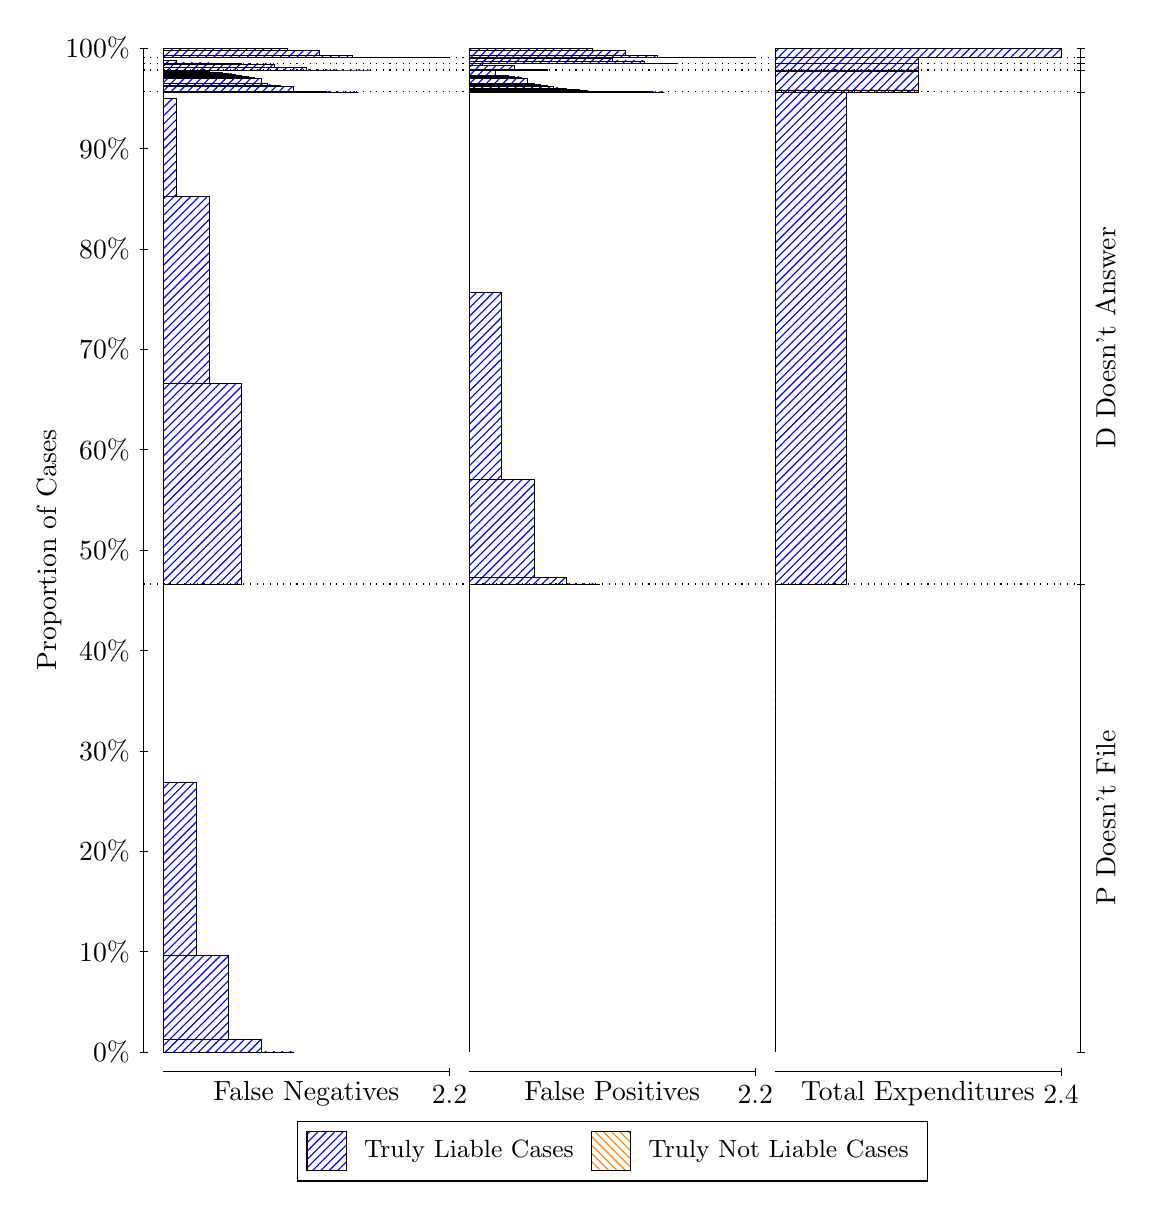
\begin{tikzpicture}
\draw[black, very thin] (1.5,1.75) -- (1.5,14.5);
\node[rotate=90, anchor=center] at (0.3, 8.125) {Proportion of Cases};
\draw[black, very thin] (1.45,1.75) -- (1.55,1.75);
\node[anchor=east] at (1.45, 1.75) {0\%};
\draw[black, very thin] (1.45,3.025) -- (1.55,3.025);
\node[anchor=east] at (1.45, 3.025) {10\%};
\draw[black, very thin] (1.45,4.3) -- (1.55,4.3);
\node[anchor=east] at (1.45, 4.3) {20\%};
\draw[black, very thin] (1.45,5.575) -- (1.55,5.575);
\node[anchor=east] at (1.45, 5.575) {30\%};
\draw[black, very thin] (1.45,6.85) -- (1.55,6.85);
\node[anchor=east] at (1.45, 6.85) {40\%};
\draw[black, very thin] (1.45,8.125) -- (1.55,8.125);
\node[anchor=east] at (1.45, 8.125) {50\%};
\draw[black, very thin] (1.45,9.4) -- (1.55,9.4);
\node[anchor=east] at (1.45, 9.4) {60\%};
\draw[black, very thin] (1.45,10.675) -- (1.55,10.675);
\node[anchor=east] at (1.45, 10.675) {70\%};
\draw[black, very thin] (1.45,11.95) -- (1.55,11.95);
\node[anchor=east] at (1.45, 11.95) {80\%};
\draw[black, very thin] (1.45,13.225) -- (1.55,13.225);
\node[anchor=east] at (1.45, 13.225) {90\%};
\draw[black, very thin] (1.45,14.5) -- (1.55,14.5);
\node[anchor=east] at (1.45, 14.5) {100\%};

\draw[black, very thin] (13.4,1.75) -- (13.4,14.5);
\draw[black, very thin] (13.35,1.75) -- (13.45,1.75);
\node[anchor=west] at (13.35, 1.75) {};
\draw[black, very thin] (13.35,7.693) -- (13.45,7.693);
\node[anchor=west] at (13.35, 7.693) {};
\draw[black, very thin] (13.35,13.944) -- (13.45,13.944);
\node[anchor=west] at (13.35, 13.944) {};
\draw[black, very thin] (13.35,14.221) -- (13.45,14.221);
\node[anchor=west] at (13.35, 14.221) {};
\draw[black, very thin] (13.35,14.305) -- (13.45,14.305);
\node[anchor=west] at (13.35, 14.305) {};
\draw[black, very thin] (13.35,14.377) -- (13.45,14.377);
\node[anchor=west] at (13.35, 14.377) {};
\draw[black, very thin] (13.35,14.5) -- (13.45,14.5);
\node[anchor=west] at (13.35, 14.5) {};

\draw[black, very thin, pattern color=blue, pattern=north east lines] (1.75,1.75) rectangle (3.4015,1.7516);
\draw[black, very thin, pattern color=blue, pattern=north east lines] (1.75,1.7516) rectangle (2.9886,1.9119);
\draw[black, very thin, pattern color=blue, pattern=north east lines] (1.75,1.9119) rectangle (2.5758,2.9735);
\draw[black, very thin, pattern color=blue, pattern=north east lines] (1.75,2.9735) rectangle (2.1629,5.1734);
\draw[black, very thin, pattern color=orange, pattern=north west lines] (1.75,5.1734) rectangle (1.75,5.1734);
\draw[black, very thin, pattern color=blue, pattern=north east lines] (1.75,5.1734) rectangle (1.75,7.693);
\draw[black, very thin, pattern color=blue, pattern=north east lines] (1.75,7.693) rectangle (2.7409,10.241);
\draw[black, very thin, pattern color=blue, pattern=north east lines] (1.75,10.241) rectangle (2.328,12.613);
\draw[black, very thin, pattern color=blue, pattern=north east lines] (1.75,12.613) rectangle (1.9152,13.857);
\draw[black, very thin, pattern color=orange, pattern=north west lines] (1.75,13.857) rectangle (1.75,13.857);
\draw[black, very thin, pattern color=blue, pattern=north east lines] (1.75,13.857) rectangle (1.75,13.944);
\draw[black, very thin, pattern color=blue, pattern=north east lines] (1.75,13.944) rectangle (4.2273,13.944);
\draw[black, very thin, pattern color=blue, pattern=north east lines] (1.75,13.944) rectangle (4.0621,13.944);
\draw[black, very thin, pattern color=blue, pattern=north east lines] (1.75,13.944) rectangle (3.897,13.944);
\draw[black, very thin, pattern color=blue, pattern=north east lines] (1.75,13.944) rectangle (3.8144,13.947);
\draw[black, very thin, pattern color=blue, pattern=north east lines] (1.75,13.947) rectangle (3.7318,13.947);
\draw[black, very thin, pattern color=blue, pattern=north east lines] (1.75,13.947) rectangle (3.6492,13.948);
\draw[black, very thin, pattern color=blue, pattern=north east lines] (1.75,13.948) rectangle (3.5667,13.948);
\draw[black, very thin, pattern color=blue, pattern=north east lines] (1.75,13.948) rectangle (3.4841,13.949);
\draw[black, very thin, pattern color=blue, pattern=north east lines] (1.75,13.949) rectangle (3.4015,14.012);
\draw[black, very thin, pattern color=blue, pattern=north east lines] (1.75,14.012) rectangle (3.3189,14.014);
\draw[black, very thin, pattern color=blue, pattern=north east lines] (1.75,14.014) rectangle (3.2364,14.014);
\draw[black, very thin, pattern color=blue, pattern=north east lines] (1.75,14.014) rectangle (3.2364,14.029);
\draw[black, very thin, pattern color=blue, pattern=north east lines] (1.75,14.029) rectangle (3.1538,14.031);
\draw[black, very thin, pattern color=blue, pattern=north east lines] (1.75,14.031) rectangle (3.0712,14.046);
\draw[black, very thin, pattern color=blue, pattern=north east lines] (1.75,14.046) rectangle (3.0712,14.046);
\draw[black, very thin, pattern color=blue, pattern=north east lines] (1.75,14.046) rectangle (2.9886,14.115);
\draw[black, very thin, pattern color=blue, pattern=north east lines] (1.75,14.115) rectangle (2.9061,14.125);
\draw[black, very thin, pattern color=blue, pattern=north east lines] (1.75,14.125) rectangle (2.8235,14.126);
\draw[black, very thin, pattern color=blue, pattern=north east lines] (1.75,14.126) rectangle (2.8235,14.142);
\draw[black, very thin, pattern color=blue, pattern=north east lines] (1.75,14.142) rectangle (2.7409,14.154);
\draw[black, very thin, pattern color=blue, pattern=north east lines] (1.75,14.154) rectangle (2.6583,14.17);
\draw[black, very thin, pattern color=blue, pattern=north east lines] (1.75,14.17) rectangle (2.6583,14.171);
\draw[black, very thin, pattern color=blue, pattern=north east lines] (1.75,14.171) rectangle (2.5758,14.182);
\draw[black, very thin, pattern color=blue, pattern=north east lines] (1.75,14.182) rectangle (2.4932,14.186);
\draw[black, very thin, pattern color=blue, pattern=north east lines] (1.75,14.186) rectangle (2.4932,14.19);
\draw[black, very thin, pattern color=blue, pattern=north east lines] (1.75,14.19) rectangle (2.4106,14.194);
\draw[black, very thin, pattern color=blue, pattern=north east lines] (1.75,14.194) rectangle (2.4106,14.195);
\draw[black, very thin, pattern color=blue, pattern=north east lines] (1.75,14.195) rectangle (2.328,14.204);
\draw[black, very thin, pattern color=blue, pattern=north east lines] (1.75,14.204) rectangle (2.2455,14.206);
\draw[black, very thin, pattern color=blue, pattern=north east lines] (1.75,14.206) rectangle (2.2455,14.208);
\draw[black, very thin, pattern color=blue, pattern=north east lines] (1.75,14.208) rectangle (2.1629,14.212);
\draw[black, very thin, pattern color=blue, pattern=north east lines] (1.75,14.212) rectangle (2.0803,14.212);
\draw[black, very thin, pattern color=blue, pattern=north east lines] (1.75,14.212) rectangle (2.0803,14.214);
\draw[black, very thin, pattern color=blue, pattern=north east lines] (1.75,14.214) rectangle (1.9977,14.217);
\draw[black, very thin, pattern color=blue, pattern=north east lines] (1.75,14.217) rectangle (1.9152,14.218);
\draw[black, very thin, pattern color=blue, pattern=north east lines] (1.75,14.218) rectangle (1.8326,14.219);
\draw[black, very thin, pattern color=orange, pattern=north west lines] (1.75,14.219) rectangle (1.75,14.219);
\draw[black, very thin, pattern color=blue, pattern=north east lines] (1.75,14.219) rectangle (1.75,14.221);
\draw[black, very thin, pattern color=blue, pattern=north east lines] (1.75,14.221) rectangle (4.3924,14.221);
\draw[black, very thin, pattern color=blue, pattern=north east lines] (1.75,14.221) rectangle (3.9795,14.221);
\draw[black, very thin, pattern color=blue, pattern=north east lines] (1.75,14.221) rectangle (3.5667,14.25);
\draw[black, very thin, pattern color=blue, pattern=north east lines] (1.75,14.25) rectangle (3.1538,14.298);
\draw[black, very thin, pattern color=blue, pattern=north east lines] (1.75,14.298) rectangle (2.7409,14.305);
\draw[black, very thin, pattern color=orange, pattern=north west lines] (1.75,14.305) rectangle (1.75,14.305);
\draw[black, very thin, pattern color=blue, pattern=north east lines] (1.75,14.305) rectangle (2.7409,14.305);
\draw[black, very thin, pattern color=blue, pattern=north east lines] (1.75,14.305) rectangle (2.328,14.31);
\draw[black, very thin, pattern color=blue, pattern=north east lines] (1.75,14.31) rectangle (1.9152,14.346);
\draw[black, very thin, pattern color=orange, pattern=north west lines] (1.75,14.346) rectangle (1.75,14.346);
\draw[black, very thin, pattern color=blue, pattern=north east lines] (1.75,14.346) rectangle (1.75,14.377);
\draw[black, very thin, pattern color=blue, pattern=north east lines] (1.75,14.377) rectangle (5.3833,14.377);
\draw[black, very thin, pattern color=blue, pattern=north east lines] (1.75,14.377) rectangle (4.9705,14.377);
\draw[black, very thin, pattern color=blue, pattern=north east lines] (1.75,14.377) rectangle (4.5576,14.378);
\draw[black, very thin, pattern color=blue, pattern=north east lines] (1.75,14.378) rectangle (4.1447,14.404);
\draw[black, very thin, pattern color=blue, pattern=north east lines] (1.75,14.404) rectangle (3.7318,14.468);
\draw[black, very thin, pattern color=blue, pattern=north east lines] (1.75,14.468) rectangle (3.3189,14.497);
\draw[black, very thin, pattern color=blue, pattern=north east lines] (1.75,14.497) rectangle (2.9061,14.5);
\draw[black, very thin, pattern color=blue, pattern=north east lines] (1.75,14.5) rectangle (2.4932,14.5);
\draw[black, very thin, pattern color=blue, pattern=north east lines] (1.75,14.5) rectangle (2.0803,14.5);
\draw[black, very thin, pattern color=orange, pattern=north west lines] (1.75,14.5) rectangle (1.75,14.5);
\draw[black, very thin, pattern color=orange, pattern=north west lines] (5.6333,1.75) rectangle (5.6333,1.75);
\draw[black, very thin, pattern color=blue, pattern=north east lines] (5.6333,1.75) rectangle (5.6333,7.693);
\draw[black, very thin, pattern color=orange, pattern=north west lines] (5.6333,7.693) rectangle (7.2848,7.693);
\draw[black, very thin, pattern color=blue, pattern=north east lines] (5.6333,7.693) rectangle (7.2848,7.6938);
\draw[black, very thin, pattern color=blue, pattern=north east lines] (5.6333,7.6938) rectangle (6.872,7.7803);
\draw[black, very thin, pattern color=blue, pattern=north east lines] (5.6333,7.7803) rectangle (6.4591,9.0243);
\draw[black, very thin, pattern color=blue, pattern=north east lines] (5.6333,9.0243) rectangle (6.0462,11.396);
\draw[black, very thin, pattern color=blue, pattern=north east lines] (5.6333,11.396) rectangle (5.6333,13.944);
\draw[black, very thin, pattern color=orange, pattern=north west lines] (5.6333,13.944) rectangle (8.1106,13.944);
\draw[black, very thin, pattern color=blue, pattern=north east lines] (5.6333,13.944) rectangle (8.1106,13.944);
\draw[black, very thin, pattern color=orange, pattern=north west lines] (5.6333,13.944) rectangle (7.9455,13.944);
\draw[black, very thin, pattern color=blue, pattern=north east lines] (5.6333,13.944) rectangle (7.9455,13.945);
\draw[black, very thin, pattern color=orange, pattern=north west lines] (5.6333,13.945) rectangle (7.7803,13.945);
\draw[black, very thin, pattern color=blue, pattern=north east lines] (5.6333,13.945) rectangle (7.7803,13.945);
\draw[black, very thin, pattern color=blue, pattern=north east lines] (5.6333,13.945) rectangle (7.6977,13.946);
\draw[black, very thin, pattern color=orange, pattern=north west lines] (5.6333,13.946) rectangle (7.6152,13.946);
\draw[black, very thin, pattern color=blue, pattern=north east lines] (5.6333,13.946) rectangle (7.6152,13.946);
\draw[black, very thin, pattern color=blue, pattern=north east lines] (5.6333,13.946) rectangle (7.5326,13.947);
\draw[black, very thin, pattern color=orange, pattern=north west lines] (5.6333,13.947) rectangle (7.45,13.947);
\draw[black, very thin, pattern color=blue, pattern=north east lines] (5.6333,13.947) rectangle (7.45,13.948);
\draw[black, very thin, pattern color=blue, pattern=north east lines] (5.6333,13.948) rectangle (7.3674,13.951);
\draw[black, very thin, pattern color=orange, pattern=north west lines] (5.6333,13.951) rectangle (7.2848,13.951);
\draw[black, very thin, pattern color=blue, pattern=north east lines] (5.6333,13.951) rectangle (7.2848,13.953);
\draw[black, very thin, pattern color=blue, pattern=north east lines] (5.6333,13.953) rectangle (7.2023,13.957);
\draw[black, very thin, pattern color=orange, pattern=north west lines] (5.6333,13.957) rectangle (7.1197,13.957);
\draw[black, very thin, pattern color=blue, pattern=north east lines] (5.6333,13.957) rectangle (7.1197,13.961);
\draw[black, very thin, pattern color=blue, pattern=north east lines] (5.6333,13.961) rectangle (7.0371,13.97);
\draw[black, very thin, pattern color=orange, pattern=north west lines] (5.6333,13.97) rectangle (6.9545,13.97);
\draw[black, very thin, pattern color=blue, pattern=north east lines] (5.6333,13.97) rectangle (6.9545,13.971);
\draw[black, very thin, pattern color=blue, pattern=north east lines] (5.6333,13.971) rectangle (6.9545,13.975);
\draw[black, very thin, pattern color=blue, pattern=north east lines] (5.6333,13.975) rectangle (6.872,13.983);
\draw[black, very thin, pattern color=orange, pattern=north west lines] (5.6333,13.983) rectangle (6.7894,13.983);
\draw[black, very thin, pattern color=blue, pattern=north east lines] (5.6333,13.983) rectangle (6.7894,13.994);
\draw[black, very thin, pattern color=blue, pattern=north east lines] (5.6333,13.994) rectangle (6.7068,14.01);
\draw[black, very thin, pattern color=blue, pattern=north east lines] (5.6333,14.01) rectangle (6.6242,14.023);
\draw[black, very thin, pattern color=blue, pattern=north east lines] (5.6333,14.023) rectangle (6.5417,14.038);
\draw[black, very thin, pattern color=blue, pattern=north east lines] (5.6333,14.038) rectangle (6.5417,14.039);
\draw[black, very thin, pattern color=blue, pattern=north east lines] (5.6333,14.039) rectangle (6.4591,14.05);
\draw[black, very thin, pattern color=blue, pattern=north east lines] (5.6333,14.05) rectangle (6.3765,14.119);
\draw[black, very thin, pattern color=blue, pattern=north east lines] (5.6333,14.119) rectangle (6.2939,14.134);
\draw[black, very thin, pattern color=blue, pattern=north east lines] (5.6333,14.134) rectangle (6.2114,14.136);
\draw[black, very thin, pattern color=blue, pattern=north east lines] (5.6333,14.136) rectangle (6.1288,14.151);
\draw[black, very thin, pattern color=blue, pattern=north east lines] (5.6333,14.151) rectangle (6.1288,14.151);
\draw[black, very thin, pattern color=blue, pattern=north east lines] (5.6333,14.151) rectangle (6.0462,14.152);
\draw[black, very thin, pattern color=blue, pattern=north east lines] (5.6333,14.152) rectangle (5.9636,14.216);
\draw[black, very thin, pattern color=blue, pattern=north east lines] (5.6333,14.216) rectangle (5.8811,14.217);
\draw[black, very thin, pattern color=blue, pattern=north east lines] (5.6333,14.217) rectangle (5.7985,14.217);
\draw[black, very thin, pattern color=blue, pattern=north east lines] (5.6333,14.217) rectangle (5.7159,14.218);
\draw[black, very thin, pattern color=blue, pattern=north east lines] (5.6333,14.218) rectangle (5.6333,14.221);
\draw[black, very thin, pattern color=orange, pattern=north west lines] (5.6333,14.221) rectangle (6.6242,14.221);
\draw[black, very thin, pattern color=blue, pattern=north east lines] (5.6333,14.221) rectangle (6.6242,14.228);
\draw[black, very thin, pattern color=blue, pattern=north east lines] (5.6333,14.228) rectangle (6.2114,14.276);
\draw[black, very thin, pattern color=blue, pattern=north east lines] (5.6333,14.276) rectangle (5.7985,14.305);
\draw[black, very thin, pattern color=blue, pattern=north east lines] (5.6333,14.305) rectangle (5.6333,14.305);
\draw[black, very thin, pattern color=orange, pattern=north west lines] (5.6333,14.305) rectangle (8.2758,14.305);
\draw[black, very thin, pattern color=blue, pattern=north east lines] (5.6333,14.305) rectangle (8.2758,14.307);
\draw[black, very thin, pattern color=blue, pattern=north east lines] (5.6333,14.307) rectangle (7.8629,14.336);
\draw[black, very thin, pattern color=blue, pattern=north east lines] (5.6333,14.336) rectangle (7.45,14.372);
\draw[black, very thin, pattern color=blue, pattern=north east lines] (5.6333,14.372) rectangle (7.0371,14.377);
\draw[black, very thin, pattern color=blue, pattern=north east lines] (5.6333,14.377) rectangle (6.6242,14.377);
\draw[black, very thin, pattern color=orange, pattern=north west lines] (5.6333,14.377) rectangle (9.2667,14.377);
\draw[black, very thin, pattern color=blue, pattern=north east lines] (5.6333,14.377) rectangle (9.2667,14.377);
\draw[black, very thin, pattern color=blue, pattern=north east lines] (5.6333,14.377) rectangle (8.8538,14.377);
\draw[black, very thin, pattern color=orange, pattern=north west lines] (5.6333,14.377) rectangle (8.8538,14.377);
\draw[black, very thin, pattern color=blue, pattern=north east lines] (5.6333,14.377) rectangle (8.8538,14.377);
\draw[black, very thin, pattern color=blue, pattern=north east lines] (5.6333,14.377) rectangle (8.4409,14.378);
\draw[black, very thin, pattern color=orange, pattern=north west lines] (5.6333,14.378) rectangle (8.4409,14.378);
\draw[black, very thin, pattern color=blue, pattern=north east lines] (5.6333,14.378) rectangle (8.4409,14.38);
\draw[black, very thin, pattern color=blue, pattern=north east lines] (5.6333,14.38) rectangle (8.028,14.38);
\draw[black, very thin, pattern color=orange, pattern=north west lines] (5.6333,14.38) rectangle (8.028,14.38);
\draw[black, very thin, pattern color=blue, pattern=north east lines] (5.6333,14.38) rectangle (8.028,14.409);
\draw[black, very thin, pattern color=blue, pattern=north east lines] (5.6333,14.409) rectangle (7.6152,14.409);
\draw[black, very thin, pattern color=orange, pattern=north west lines] (5.6333,14.409) rectangle (7.6152,14.409);
\draw[black, very thin, pattern color=blue, pattern=north east lines] (5.6333,14.409) rectangle (7.6152,14.473);
\draw[black, very thin, pattern color=blue, pattern=north east lines] (5.6333,14.473) rectangle (7.2023,14.499);
\draw[black, very thin, pattern color=blue, pattern=north east lines] (5.6333,14.499) rectangle (6.7894,14.5);
\draw[black, very thin, pattern color=blue, pattern=north east lines] (5.6333,14.5) rectangle (6.3765,14.5);
\draw[black, very thin, pattern color=blue, pattern=north east lines] (5.6333,14.5) rectangle (5.9636,14.5);
\draw[black, very thin, pattern color=orange, pattern=north west lines] (9.5167,1.75) rectangle (9.5167,1.75);
\draw[black, very thin, pattern color=blue, pattern=north east lines] (9.5167,1.75) rectangle (9.5167,7.693);
\draw[black, very thin, pattern color=orange, pattern=north west lines] (9.5167,7.693) rectangle (10.425,7.693);
\draw[black, very thin, pattern color=blue, pattern=north east lines] (9.5167,7.693) rectangle (10.425,13.944);
\draw[black, very thin, pattern color=orange, pattern=north west lines] (9.5167,13.944) rectangle (11.333,13.944);
\draw[black, very thin, pattern color=blue, pattern=north east lines] (9.5167,13.944) rectangle (11.333,13.967);
\draw[black, very thin, pattern color=orange, pattern=north west lines] (9.5167,13.967) rectangle (11.333,13.967);
\draw[black, very thin, pattern color=blue, pattern=north east lines] (9.5167,13.967) rectangle (11.333,14.208);
\draw[black, very thin, pattern color=orange, pattern=north west lines] (9.5167,14.208) rectangle (11.333,14.208);
\draw[black, very thin, pattern color=blue, pattern=north east lines] (9.5167,14.208) rectangle (11.333,14.221);
\draw[black, very thin, pattern color=orange, pattern=north west lines] (9.5167,14.221) rectangle (11.333,14.221);
\draw[black, very thin, pattern color=blue, pattern=north east lines] (9.5167,14.221) rectangle (11.333,14.305);
\draw[black, very thin, pattern color=orange, pattern=north west lines] (9.5167,14.305) rectangle (11.333,14.305);
\draw[black, very thin, pattern color=blue, pattern=north east lines] (9.5167,14.305) rectangle (11.333,14.377);
\draw[black, very thin, pattern color=orange, pattern=north west lines] (9.5167,14.377) rectangle (13.15,14.377);
\draw[black, very thin, pattern color=blue, pattern=north east lines] (9.5167,14.377) rectangle (13.15,14.379);
\draw[black, very thin, pattern color=orange, pattern=north west lines] (9.5167,14.379) rectangle (13.15,14.379);
\draw[black, very thin, pattern color=blue, pattern=north east lines] (9.5167,14.379) rectangle (13.15,14.5);
\draw[black, dotted] (1.5,7.693) -- (13.4,7.693);
\draw[black, dotted] (1.5,13.944) -- (13.4,13.944);
\draw[black, dotted] (1.5,14.221) -- (13.4,14.221);
\draw[black, dotted] (1.5,14.305) -- (13.4,14.305);
\draw[black, dotted] (1.5,14.377) -- (13.4,14.377);
\draw[black, very thin] (1.75,1.5) -- (5.3833,1.5);
\node[anchor=north] at (3.5667, 1.5) {False Negatives};
\draw[black, very thin] (5.3833,1.45) -- (5.3833,1.55);
\node[anchor=north] at (5.3833, 1.45) {2.2};

\draw[black, very thin] (5.6333,1.5) -- (9.2667,1.5);
\node[anchor=north] at (7.45, 1.5) {False Positives};
\draw[black, very thin] (9.2667,1.45) -- (9.2667,1.55);
\node[anchor=north] at (9.2667, 1.45) {2.2};

\draw[black, very thin] (9.5167,1.5) -- (13.15,1.5);
\node[anchor=north] at (11.333, 1.5) {Total Expenditures};
\draw[black, very thin] (13.15,1.45) -- (13.15,1.55);
\node[anchor=north] at (13.15, 1.45) {2.4};

\node[black, centered, rotate=90] at (13.72, 4.7215) {P Doesn't File};
\node[black, centered, rotate=90] at (13.72, 10.819) {D Doesn't Answer};





\draw (7.449999999999999,1.5) node[draw=none] (baseCoordinate) {};
\begin{scope}[align=center]
        \matrix[scale=0.5, draw=black, below=0.5cm of baseCoordinate, nodes={draw}, column sep=0.1cm]{
            \node[rectangle, draw, minimum width=0.5cm, minimum height=0.5cm, pattern=north east lines, pattern color=blue] {}; &
            \node[draw=none, font=\small] (B) {Truly Liable Cases}; &
            \node[rectangle, draw, minimum width=0.5cm, minimum height=0.5cm, pattern=north west lines, pattern color=orange] {}; &
            \node[draw=none, font=\small] (B) {Truly Not Liable Cases}; \\
            };
\end{scope}

\end{tikzpicture}
\end{document}